% !TeX spellcheck = fr_FR
\section{\Duo}
La traduction de \Duo{} \begin{CJK*}{UTF8}{bsmi}剁\end{CJK*} fait référence au terme de cuisine \textit{émincer} qui évoque en quelque sorte un mouvement répété et une coupe utilisant une partie de la lame plus éloignée de la pointe que \Pi{}. Le mouvement lui-même est la combinaison d'une extension vers l'avant et d'une sorte de cisaillement, comme lorsqu'on utilise un gros couteau de cuisine pour émincer des herbes aromatiques ou des légumes.

Dans la tradition du \Yangjia{} \Michuan{}, \Duo{} est typiquement réalisé avec les deux bras étendus pratiquement dans l'alignement de la lame de l'épée (fig. \ref{fig:duo_full}). 


\begin{figure}[ht]
	\centering
	
	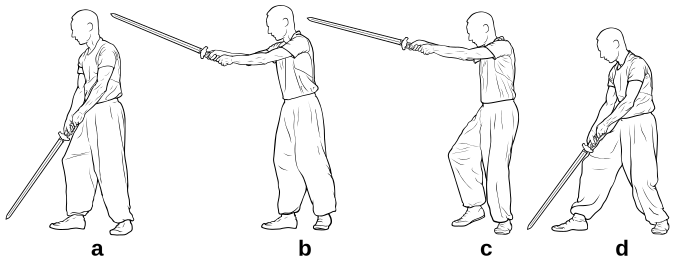
\includegraphics[width=1.00\textwidth]{../../Images/JibenJianfa/Duo/Duo.pdf}
	\caption[\Duo{} en avançant]{\Duo{} en avançant. À partir d'une garde basse (a), lever l'épée en transférant le poids sur le pied droit (b), inverser la polarité entre les mains et transférer le poids à nouveau sur le pied gauche (c), puis abaisser l'épée tout en s'enracinant dans la jambe gauche et en avançant le le pied droit.}
	\label{fig:duo_full}
\end{figure} 

Bien que les deux mains soient en contact avec la poignée, il ne faut pas confondre cette position avec une prise à deux mains de la fusée. À la montée et en avançant, la main droite tient l'épée tandis que la main gauche donne la structure et transmet la puissance en poussant sur le pommeau suivant la direction de la lame. La force est générée par le transfert de poids de la jambe arrière à la jambe avant. Elle est transmise à l'épée par la main gauche/arrière pendant que la main droite/avant équilibre exactement et passivement cette force pour générer la technique sans effort. Cette combinaison du rôle passif de la main droite et de l'action de la main gauche crée une polarité induisant un mouvement de l'épée perpendiculaire à l'axe du bras droit. Une connexion effective entre la taille et l'épée permet alors l'expression explosive de la technique \Duo{}. Cette méthode fait en quelque sorte écho aux préceptes trouvés dans le \JianJing{} précisant que, en manipulant une épée à deux mains, la puissance est dans la taille, puis dans la main arrière, et finalement dans la main avant. À la descente, les rôles des deux mains sont inversés et en reculant, bien que les forces combinées soient identiques, la main droite est active en montant, et passive en descendant (fig. \ref{fig:duo_detail}). Une règle générale est, qu'on avance ou qu'on recule, que la main active est celle qui se trouve du même côté que le pied qu'on déplace.

\begin{figure}[ht]
	\centering
	
	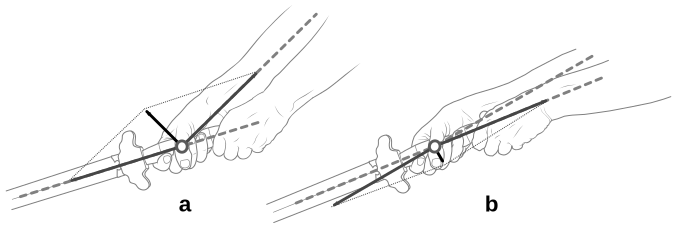
\includegraphics[width=1.00\textwidth]{../../Images/JibenJianfa/Duo/DuoDetail.pdf}
	\caption[Équilibre des forces dans le \Duo{}]{(a) Pour réaliser un \Duo{} ascendant vers l'avant, la main gauche pousse la poignée dans la direction de la pointe de la lame tandis que le bras droit équilibre passivement cette poussée. En raison de l'angle entre la direction de poussée et le bras droit, il en résulte une force perpendiculaire au bras droit qui fait monter l'épée. En reculant, les même forces s'appliquent mais la main droite tire activement l'épée tandis que la gauche équilibre passivement cette action. \\
	(b) Pour réaliser un \Duo{} descendant vers l'avant, la main droite pousse la poignée vers l'avant tandis que la main gauche la retient passivement en équilibrant la force de poussée. La force résultante, perpendiculaire à l'axe du bras gauche, tire l'épée vers le bas. Pour un déplacement à reculons, la main gauche tire l'épée tandis que la droite est passive.
	}
	\label{fig:duo_detail}
\end{figure} 


Puisqu'en cuisine, les aromates et légumes sont généralement émincés en coupant vers le bas, on peut argumenter que la phase active de \Duo{} serait la phase descendante. Toutefois, l'examen attentif du mouvement réel d'un couteau de cuisine lorsqu'on émince montre que la phase active correspond en réalité à la phase ascendante de \Duo{} en avançant. La seule différence est que dans le cas du couteau, la pointe reste au contact du plan de travail tandis que la pointe de l'épée monte, mais dans les deux cas, le tranchant suit un mouvement similaire relativement à la pointe.
Il est cependant parfaitement possible d'être actif pendant les deux phases, la phase passive étant en fait le mouvement de transition entre la montée et la descente. Ainsi, \Duo{} peut être un estoc ou une coupe en montant aussi bien qu'en descendant. Cette technique peut même, combinée à \Mo{}, être une action sur la lame de l'adversaire, soit en montant pour intercepter et dévier, soit en descendant pour un froissement. 

Il est important de noter ici que, puisque les deux mains sont en contact avec la poignée, l'épée est toujours en ligne avec l'axe du corps. Cet axe est plutôt du côté gauche dans la position, garde basse et appui pied arrière, qui précède la phase ascendante de \Duo{} en avançant. Puis, pendant la phase montante du mouvement, l'axe se décale vers la droite pour revenir à gauche en redescendant. Par exemple, pendant l'application dévier/froisser de \Duo{} combiné à \Mo{}, le transfert de poids vers la jambe droite pendant la parade haute écarte légèrement vers l'extérieur la pointe de l'adversaire, permettant de diriger ensuite naturellement le froissement vers le centre de l'épée adverse, la déviant plus loin encore et ouvrant la voie à la touche tout en évitant une contre-attaque.

\fiche{The simplest application of \Duo{} starts with a lower guard as an invitation for the opponent to prepare an attack. We can then engage and deflect with a \Duo{} before placing our riposte or we may take advantage of the explosive nature of the movement and use an offensive \Duo{} to thrust directly during the opponent's preparation.
	\Duo{} is often performed in series of two to three movements, not more to avoid predictability, as seen for the double-handed version in the \Kunlun{} form. We can usually identify three periods in these series: The first \Duo{} movement would intercept an incoming attack, either a \Pi{} or a \Hua{} cut from above or a high level \Ci{} thrust.Then, the second one will deflect the opponent's blade to open the way for the third \Duo{} thrust. Of course, this is not a fixed pattern, and the first movement can be followed by any appropriate technique depending on the circumstances. For instance, instead of deflecting, the second step may accompany the opponent's blade to control it while entering to prepare the riposte.}

Bien que le mouvement classique soit réalisé à deux mains, il est aussi possible de réaliser un \Duo{} avec une seule main. Dans ce cas, le talon de la main joue le même rôle que la main arrière dans la version à deux mains, et les trois premiers doigts \textemdash{} index, majeur et pouce \textemdash{} jouent le rôle de la main avant. 

Pendant la phase ascendante, la poignée de l'épée est poussée vers l'avant par le talon de la main et simultanément retenue par les doigts. Grâce à une bonne structure de la position de garde, il est alors possible, même à une seule main, de rapidement lever l'épée sans effort d'une position basse à une position haute pour estoquer ou engager.

\fiche{When descending, the fore fingers relax their grip while the ring and little fingers are tightened to pull the handle. Some intention should be put at the base of the index to gently push the handle downwards in the forward direction. The resulting structure allows to capture and deflect the centre of the opponent's sword by shearing or to perform a powerful cut while retreating.}

L'alignement de l'épée est assez similaire à ce qu'il est dans la version à deux main, la pointe de la lame en ligne avec l'axe du corps. Toutefois, la structure est moins solide qu'avec \Duo{} à deux mains, et il en résulte des froissements moins puissants. Cependant, cette version du mouvement est utile pour engager rapidement la lame adverse ou pour une attaque soudaine en partant d'une garde basse.